\documentclass{beamer}
\usepackage{tikz}

\tikzset{onslide/.code args={<#1>#2}{%
  \only<#1>{\pgfkeysalso{#2}} % \pgfkeysalso doesn't change the path
}}

\begin{document}

\begin{frame}

  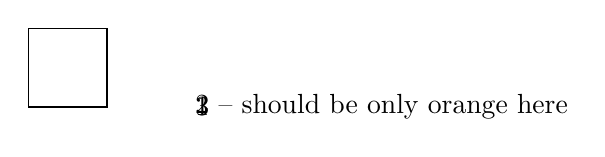
\begin{tikzpicture}
    \draw [onslide=<2>{fill=orange}] (0,0) rectangle (1,1);
    \uncover<1>{\node at (2,0) [anchor=west] {1};}
    \uncover<2>{\node at (2,0) [anchor=west] {2 -- should be only orange here};}
    \uncover<3>{\node at (2,0) [anchor=west] {3};}
  \end{tikzpicture}

\end{frame}

\end{document}
